% This document explores our implementation with a focus on looking at the exact timeline of implementation by flushing out the Gantt chart's timeline into more clear and concise week by week evaluations. The points of design for this document includes the searchable encryption algorithm, Research of parallelization, and Benchmarking comparisons between other similar algorithm implementations. Each of these major sections contain sub parts that pertain to specific problems we may run into during implementation and how we plan to overcome said problems.

\chapter{Design Document}

% Research paper structure
% 1. Introduction / overview
% 2. Projects
% 	a. Searchable encryption
%   b. Case Study 1
%   c. Case study 2
% 3. Conclusion

\section{Introduction}

\subsection{ Purpose }

The purpose of this document is to specify the system design for the Privacy Preserving Cloud project, and to give an estimated schedule.


\subsection{ Summary }


% The goal of this project is 
% a) demonstrate usability of SSE
% b) research refinements to Cash-DSSE
% c) provide benchmarks of our variations vs baseline and vs IM-DSSE and Clusion


% insert one-sentence summary of the project and its goals here
% ...

Our project is centered around the searchable encryption algorithm implementation.
The remaining parts of the project are a series of case studies to investigate various aspects of this central core:
integrating it with email systems,
finding ways to speed the algorithm up, etc. 
These parts can all proceed more or less independently once we have the core working.
Finally, we will benchmark our results against our baseline implementation, and against two other SSE implementations.

%star-shaped

Of all the parts of the project, the first part --- implementing the core SSE algorithm \ref{subsec:sse} --- is the most well-understood, since the algorithm has already been completely described in a paper.
The email integration part (\ref{subsec:email}) is also more of an engineering challenge than a research challenge. 
%This is reflected in the largely concrete description of these parts.
The remaining parts are more research-oriented and are accordingly described in terms of the research question and what avenues we intend to explore to answer it.

Thus, the design set forth here is not set in stone.
We expect to have be flexible and to adapt our plan to where the research leads us. 

% aspirational, not ...


\section{ Definitions }

\paragraph*{\textbf{searchable encryption scheme}} An algorithm which allows a client to efficiently search encrypted documents on a remote server.

\paragraph*{\textbf{Cash-DSSE}} The SSE algorithm described by Cash et al. in \cite{cash14}

\paragraph*{\textbf{IM-DSSE}} The SSE algorithm described by Yavuz and Guarjardo in \cite{yavuz15}


% etc


\section{ Project components }

% Design concerns / constrains

% From the assignment description:
% > In the design document each member will write up the design of each of the three pieces he/she will be owning and managing for the remainder of the year. The entire group will then combine individual work into one full document, framed with a proper introduction and conclusion. You will be graded as a group as you were with the requirements document.
% > This document should include the full *HOW* of your system including your API, your timeline, necessary testing information, etc. Use this document as a guide to plan the rest of the year's work. Remember, a week of debugging can save you 20 minutes of planning! Plan the work, work the plan.



Andrew Ekstedt will be primarily responsible for \ref{subsec:sse} and \ref{subsec:dumbserver}.
Scott Merrill will be primarily responsible for \ref{subsec:parallel} and \ref{subsec:size}.
Scott Russell will be primarily responsible for \ref{subsec:email} and \ref{subsec:benchmark}.

\subsection{ Searchable encryption algorithm }
\label{subsec:sse}

% Andrew Ekstedt

% gonnna do cash

% - written in C++
% - operations: search, update, delete
% - using tomcrypt for crypto primitives
% - using AES-128-CTR for encryption scheme
% - using HMAC-SHA1 for variable-length PRF(?)
% - using ZeroMQ for client-server communication

The heart of our project is the searchable encryption algorithm (SSE).
We plan to implement the algorithm described in \cite{cash14} (hereafter Cash-DSSE).

The initial implementation of the SSE will constitute a baseline which we will compare subsequent variations to. 
See subsection \ref{subsec:benchmark}.

% Prior work: our client designed and implemented a different SSE algorithm \cite{yavuz15} in 2015-2016 (hereafter IM-DSSE). Cash-DSSE is asymptotically more efficient than IM-DSSE, but we want to know if it is practically more efficient

There are 3 subcomponents.

\subsection{ Search algorithm }

The core subcomponent is C++ library which implements the SSE algorithm. 

It will support the following operations:
% XXX these operations should have a server half and client half
\begin{itemize}
\item \textbf{Gen} generates a secret key
\item \textbf{Setup} constructs an encrypted search index from an initial set of files
\item \textbf{Search} takes a search keyword and returns a list of matching files
\item \textbf{Update} takes an operation (add, delete), a file id, and a list of keywords and performs the appropriate action
\end{itemize}

Each of these operations (except Gen) will be split into client-side and server-side halves.
The client side operation will perform some computations, construct a message, and send it to the server.
Upon receiving a message, the server will unpack the message, 
call the appropriate function, do some computations,
and send a response back to the client.

Cash-DSSE relies on two cryptographic primitives:
a symmetric encryption scheme and a variable-length input PRF.
We plan to use AES-128-CTR for the encryption scheme and HMAC-SHA256 for the PRF.
Implementations of both algorithms will be supplied by the tomcrypt \cite{tomcrypt} library.

The client and server will be written in C++ and exchange messages with the ZeroMQ library.

\subsection{ Server program }

The server program is a daemon which responds to client requests.
The server is responsible for maintaining the encrypted files and encrypted search index.

%- how to store files
Encrypted files will be stored on the remote filesystem in a flat directory structure.
When the client requests a file, the encrypted copy will be sent to the client and decrypted on the client side.

%- how to store index
The index will be stored as a file in an ad-hoc format.
%We prefer to use a binary format which is close to how the data structures are layed out in memory over a textual format like JSON or XML because it will make subsection \ref{subsec:dumbserver} easier to implement.
Cash-DSSE combines several data structures--the main search index, which is static, and two smaller data structures to keep track of additions and deletions.
We can store these different data structures in separate files. %why?

Since these ancillary data structures tend to grow over time, we will want the server to be able to periodically reconstruct the index. % how?

\subsection{ Client program }

The client program will be a basic command-line program which talks to the server.
It will allow the user to create a search index, add and delete files, and search for a keyword.

It will be written in C++ and use the SSE library to interact with the server.

\subsection{ Case Study: Email Daemon }
\label{subsec:email}

% Goal: demonstrate usability of SSE by showing how it can be used to automatically index emails.
% Prior art: ?
% Methodology: construct a daemon which periodically downloads emails and adds them to the search index
% Measurements: speed?
% Hypothesis: we kind of take it as a given that this demonstrates usability. do we have a real hypothesis here?

The literature on SSE is primarily focused on abstract document storage. We would like to demonstrate how SSE can be used in practice by using it to build a proof-of-concept searchable email database.

% Scott Russell
Most email services we use have a vast variety of functionalities we take for granted.
Specifically, synchronization and automatic update.
When you receive a new email your email device automatically update you of this email without any manual checking on the part of the user. 
To address this expectation, we will build a background daemon which periodically download emails over POP3 and adds them to the search index using the our SSE library.
We plan to set the update rate to once every minute.
If you set this interval too small it will take away processing from server access, however making it too large will negatively affect client user accessibility to updates.
We believe that once every minute will be an effective middle ground that provides convenience with minimal impact to the server.
% XXX maybe the update interval should be phrased as a research question? we don't have any data to back up the one minute interval we assert here

\subsection {Case Study: Search Index Size Optimization}
\label{subsec:size}

% Research question: can we decrease the index size?
% Prior research: In the paper Cash gives several ways to trade off index size for search time
% Refined research question: Cash's optimizations are parameterized by the block size. What is the optimum setting for this parameter?
% Methodology: implement \Pi_{2lev}^{ptr} as described in the paper. measure index size versus time and select the optimum result
% measurements: time versus index size
% Hypothesis: ?

% Scott Merrill
The size of the index will greatly impact if this algorithm will be usable on different platforms.
For a single user on a home desktop, the size of the index may not be an issue.
When hosting this service as a form of cloud storage for multiple the index size could impact if this sort of service is even possible.
Similarly on an email server this would have the same impact.

For our project we are going to focus on trying to answer the following questions:

\begin{enumerate}
	\item Is the index size a factor for both small and large scale systems? 

In small scale situations, like our proof of concept model, the index size is irrelevant.
There will be no real concern for the time it takes for us to search or update the index.
In larger scale implementations, like an email server, the time it takes for an email to be tokenized, and then to update the index impacts the usability.
    
	\item How to be optimize the index size:
    \begin{itemize}
		\item Reducing Dictionary Retrievals
   
The encrypted dictionary (file index) is typically stored on disk, which can slow down search operations. To improve the search time we are attempt to experiment by adding identifiers to the individual blocks of the dictionary. Then we can pack these blocks together and process them as a single ciphertext. This has been proven in the Case\-DSSE paper to greatly improve search time.  

		\item Optimizing Pointers for Different Sized Dictionaries
        
Pointers are used to locate the different blocks of identifiers used for retrieval when performing search functions. There is an issue when performing search functions on very large sets of data that still result in a large amount of dictionary retrievals (even using the previously mentioned technique of condensing identifiers into fixed block sizes). To avoid this problem we can instead change the way pointers are stored depending on the size of the dictionary. for small sets we will store identifiers directly into the dictonary (without using pointers). For medium sized sets we store them as a block of pointers that point to blocks of identifiers. For large sets we need to create a form of misdirection to avoid information leakage. We can do this by storing pointers in the dictionary that points to a block of pointers, which then points to the block of identifiers.  

    \end{itemize}

  	\item How to compare with both unoptimized versions and IM-DSSE

	The main focus of this research will be to gather information based off of unit test.
    Data gathered can be used to determine what can and needs to be optimized.
    When comparing with IM-DSSE we will not only be able to do basic test cases, such as the time it takes to perform the search and update functions.
    When comparing with unoptimized versions we can perform the same sort of tests as with IM-DSSE along with tests cases when used implemented with a cloud server or email. 
\end{enumerate}



\subsection {Case Study: Parallelization}
\label{subsec:parallel}

% Research question: can we parallelize Cash-DSSE to speed it up?
% Prior work? Yes! David cash et al claim that Cash-DSSE is trivially parallelizable
% Methodology: Examine the search algorithm to see which computations are independent and can thus be computed in parallel.
% Measurements: search time
% Hypothesis: ?

% Cash et al. claim in \cite{cash14} that their scheme is trivially parallelizable. We hope to replicate this result.

% Scott Merrill
This is what we what we know about the problem: \\
Another goal we have is to discover what ways we can improve the efficiency of the system. With a client/sever system, it is possible that there are a number of actions that can be done concurrently. This will help to improve efficiency of the system as well as decrease the time spent idle. \\

What we hope/expect to find:
\begin{enumerate}
\item By using AES-CTR are looking to parallelize the encryption process. This can be accomplished by distributing chunks of consecutive blocks among processors to be encrypted in parallel. This will allows us to take advantage of multi\-core processors.
\item we will be exploring ways to decrease idle/wait time between server and client communication. This can be accomplished by experimenting with which source does the certain forms of computation. My moving more computation from the server to the client we will decrease load on the server and allow the server to process more requests. 
\end{enumerate}

This research will be largely focused on internal testing with tests cases to determine the best practice. Parameters may include: Size of dictionary, Number of clients, and Speed of the network. subsection 3.6 will outline the specific tests cases and benchmarks we will use to evaluate our experiments and to determine the effectiveness of our results. 

\subsection {Case Study: Storage-only Server}
\label{subsec:dumbserver}

%does not compute
%- using EC2

% Research question: is it feasible to move all computation to the client? how much of an impact does that have?
% Prior work? yes (find and cite)
% Methodology: move at least decryption to client. if possible, get rid of server entirely. 
% Measurement: time to search vs baseline
% Hypothesis: it will not be much slower


The initial SSE implementation (\ref{subsec:sse}) will use a client-server model where both the client and server are capable of performing arbitrary computations.
We are interested in whether it is still possible to implement the SSE when the server can only store files, not compute---and if it is, how much of a performance impact it makes.

One benefit of this kind of approach is that it increases overall security of the scheme.
The normal operation of the server upon receiving a search token and key from the client is to retrieve the relevant entries from the search index, decrypt them, and return them to the client.
This leaks some information to the server about which file ids are associated with which tokens.
The search token is scrambled, so the server doesn't learn anything useful, but it would still be better if the server couldn't see the file ids at all. 

We can do this by moving the decryption step from the server to the client; 
the server would be responsible only for fetching the relevant entries from the index and sending them back to the client.
We can probably eliminate the server's role entirely and have the client just fetch the relevant data entries from the server, assuming the data structure for the encrypted index is stored in a way that makes this easy.

%We plan to demonstrate a storage-only server by integrating with Amazon S3.

If successful, we will compare the time to search a storage-only server versus baseline. We expect that there will not be much of a difference in performance.

\subsection {Benchmarking}
\label{subsec:benchmark}

% Scott Russell
We plan to thoroughly bench our SSE implementation both during and at the conclusion of the project.
There are many different aspects of testing that will be taking place.

% Since we are using a Spiral Model for implementation we will also be testing all of these aspects of our project throughout.

There are two primary axes which we want to test against: our implementation versus other implementations, and our baseline implementation versus the variations described in subsection 3.
Our initial SSE implementation (subsection \ref{subsec:sse}) will be our baseline implementation;
we can then graph and track how well specific optimizations increase performance and be able to see in retrospect what processes improved performance the most.

\subsection {Metrics}

\paragraph {Round-trip delay}

\textit{Round-trip delay} measures the time from when the client makes a request to when it receives a response from the server.
This can be easily measured on the client by taking the difference between the time the message is send and the time is received, and requires no synchronization between the client and server.

Since latency depends on many factors it is important to do a large sample size at different times of the day using the same systems to create an accurate average latency across different implementations. 
A high-resolution clock will be used to create smaller tick periods between time stamps to provide a more accurate representation of latency. 

Since round-trip delay is impacted by network speed as well as the speed of the underlying algorithm, it will be important to test under a variety of network conditions.
We will perform each test on a slow network, such as a public Wi-Fi network, as well as a fast network, such as a wired gigabit Ethernet connection.

\paragraph {Index size} \textit{Index size} is simply the size of the encrypted index in bytes. Smaller is better.

By measuring both round-trip delay and index size we can see how variations of the SSE algorithm trade off speed and size.


\subsection {Other implementations}

To have a point of reference we will test our implementation against IM-DSSE and Clusion.

\paragraph{IM-DSSE}
IM-DSSE \cite{im-dsse} is a C++ implementation of \cite{yavuz15}, which uses a incidence matrix data structure. Because our project and IM-DSSE are both implemented in C++, but use different SSE algorithms, this should give us a direct comparison of how the two algorithms fare against each other.

\paragraph{Clusion}
Clusion \cite{clusion} is a collection of Java implementations of several SSE algorithms --- in particular, the same algorithm we are using. Because Clusion implements the same SSE algorithm as our project, but in different slower programming language, this should give us a low anchor for our other benchmarking results.

\subsection {Discussion}

Benchmarking is an important aspect of project implementation.
Although implementation of the algorithm may be correct, faulty testing can create results that fail to simulate real world situations where these algorithms would be implemented.
This is the importance of having a full range of testing benchmarks on our specific project.

The other major component of benchmark testing is in how these algorithms handle data sets.
In small data samples there is a much higher probability for inconsistent speeds based on performance of uncontrollable and not of the specific algorithm being tested.
To counteract these effects, we will be using the maximum storage capacity of our system, one that utilizes the data cap of 5 GB of our S3 Cloud Platform. Using this data set we will use a similar testing method as the Round Trip Delay, but instead of just the time between client-server-client we will include all the processing time for the algorithm to perform the search, update, or delete that was requested.
We will be able to use this information to determine the practical speeds of these three algorithms relative to one another.
The primary purpose of this stage of the project is to be able to calculate and determine algorithm speeds thus it is vital that we minimize any external variables during testing. 


%We will explore how efficiency compares to bit block size. 128 Bit Block AES will be ideal for fast network connections. We will be testing both the 128 Bit Block AES as well as a single bit block against both a fast connection (Ethernet home network) compared to an open public Wi-Fi network. (OSU Secure)

%Using this with all three separate implementations of a DSSE Algorithm will result in being able to determine which algorithm implementation has the shortest Round Trip Delay.



\section {Schedule}

We plan to have a working implementation of the basic SSE algorithm by the second week of winter term, after which each project member will work on separate projects as outlined above.
We hope to wrap those up at the end of Winter term, and to do comprehensive testing and benchmarking starting at the end of Winter term and going into Spring.
See Figure \ref{figure:gantt} for a detailed chart.

\begin{figure}
\centering
\includegraphics[angle=270,width=6.5in]{gantt.ps}
\caption{Gantt chart}
\label{figure:gantt}
\end{figure}

% Winter Week 1-3: phase 1: implement basic SSE

% Winter Week 4-10: phase 2: parallel projects

% 	- implement storage-only server
    
%     - optimize size \& parallelization
    
%     - email integration
    
% Winter Week 9-Spring week 2?: phase 3: benchmarking

% it's probably okay if some of the research ends up getting pushed to spring, as long as we have a basic working implementation and some interesting benchmark results

\section{ Conclusion }
After completion of this document we now have a better grasp on the timeframe of our implemenetation. From integration of the core SSE to benchmarking. A clear week to week plan will greatly improve accountability as well as keep our team on track to complete all project requirements by the end of the year.
